\chapter{Risk, Quality, Ethics and Sustainability}
\label{chapter:ent-risk}

% Owner: Eesh

This chapter evaluates the non-financial readiness of the proposed headset. Commercial viability of a medical device depends not only on a healthy P\&L but also on its ability to produce reliable evidence, maintain consistent manufacturing, and operate within an adequate ethical and disposability framework, reflecting the wider medical-device principle that risk management, quality management and post-market learning operate across the whole product lifecycle. The chapter therefore (i)~stress-tests the financial projections of \Cref{chapter:ent-financial} under correlated downside scenarios, (ii)~conducts a qualitative ISO~14971-style risk assessment, and (iii)~sets out the quality, ethical and lifecycle commitments that underpin the regulatory pathway in \Cref{chapter:ent-regulatory}.


\section{Scenario Analysis}
\label{sec:ent-scenarios}

The base-case sensitivity tornado in \Cref{sec:ent-weaknesses} treats each financial driver as independent. In practice, the venture's operating risks are correlated: the same Phase 1 outcomes drive both the regulatory pathway and the early adoption curve, and the Phase 3 cost-down depends on cumulative shipped volume. This section identifies the strongest correlations between levers and tests two plausible joint scenarios within the scenario-planning framework~\cite{schoemaker1995scenario}.

\subsection{Lever Correlations}

\textbf{Clinical evidence, regulation and adoption.} The strongest correlation links these three levers. EU MDR conformity assessment depends directly on providing sufficient clinical data for the device's intended use~\cite{mdr_article61}, and weaker Phase 1 validation reduces buyer confidence as well as the conformity package: uptake depends on the interaction between technology, value proposition, adopter system, organisation and wider regulatory context, rather than technical performance alone~\cite{greenhalgh2017nasss}.

\textbf{Hardware as an acquisition channel for subscription.} Hardware shipments act mainly as an acquisition channel for recurring software-subscription revenue. If early users trust NeuroScreen and the device fits institutional practice, shipments rise, subscription attach improves, churn stays low and blended ARPU is protected. If user experience is poor or the result is not trusted, adoption slows, churn rises and ARPU falls as discounts are used to retain customers.

\textbf{Adoption, unit cost and ASP.} A third correlation links adoption to unit cost and ASP. If the Phase~3 cost-down (\Cref{sec:ent-weaknesses}) fails, hardware contribution falls from approximately \pounds126 to \pounds15 per unit and Y7 EBITDA falls to approximately \pounds(690)\,k even before allowing for lower volumes. The cost risk is not independent of adoption: slower uptake reduces purchasing scale and supplier leverage, while a higher BOM forces either a higher price (which weakens grassroots adoption) or a lower margin (which worsens cash burn).

\textbf{Regulatory slip and fixed cost base.} A one-year regulatory slip extends the pre-revenue or low-revenue period while the company continues to carry technical, quality and regulatory staff. This is a realistic possibility given persistent industry concerns around MDR cost, timelines and notified-body certification delays~\cite{medtech_europe_2024}. The slip is manageable if hiring remains milestone-oriented but dangerous if the cost base has already been scaled for commercial launch.

\subsection{Best Case and Worst Case}

\textbf{Best case.} Assuming Phase 1 validation returns strong results and the EU pathway stays on schedule, the tornado levers can be approximated as adoption ramp 20\% above base, churn reduced from 10\% to 8\%, hardware ASP 10\% above base, blended ARPU 10\% above base, unit cost 10\% below base after the planned cost-down, and monthly cash burn no more than 5\% above plan. The strategic response is to use stronger traction to negotiate supplier terms, raise capital on less dilutive terms, and expand institutional partnerships rather than scaling uncontrollably.

\textbf{Worst case.} Assuming a 12-month delay on the EU regulatory pathway, expect adoption 20\% below base, churn rising from 10\% to 15\%, hardware ASP and blended ARPU falling 10--15\%, unit cost 20--30\% above base because the cost-down path slips, and monthly burn 10\% above plan. The mitigation is to either raise enough capital to survive a 12-month regulatory slip or maintain a non-dilutive grant and contingency pipeline against delay risk. Phase~3 expansion should be deferred until both unit cost and adoption KPIs sit inside their target ranges, because selling into a low-margin grassroots channel before cost-down is complete would convert growth into cash burn.


\section{Risk Management}
\label{sec:ent-risk-mgmt}

This section conducts an abbreviated qualitative risk-management process to demonstrate how the main safety, technical, clinical, operational and commercial risks associated with NeuroScreen will be identified, evaluated and mitigated. The process is adapted from ISO~14971~\cite{iso14971}, the medical-device risk-management framework used to structure hazard identification, risk estimation, risk control, residual-risk evaluation and post-market monitoring. ISO~14971 was chosen because it later supports both IRAS/REC/MHRA-style research approval and the EU MDR conformity assessment of \Cref{chapter:ent-regulatory}. Its main limitation here is that NeuroScreen is at Stage~1 of the prototype roadmap (\Cref{tab:prototype-stages}); verified bench testing, clinical investigation documentation, usability validation, supplier controls and post-market surveillance procedures are not yet available, and proportionate functional assumptions are made to allow a qualitative assessment.

\subsection{Risk Evaluation Methodology}

Risks are evaluated using a qualitative likelihood-versus-severity matrix (\Cref{fig:risk-matrices}). Numerical failure probabilities are not assignable at this stage because NeuroScreen has not yet generated clinical, field-use or post-market data. The assessment uses a \emph{risk-averse} matrix for risks that could cause clinical harm, false reassurance, unsafe user exposure, data-governance failure or regulatory rejection, because the consequence of a misleading output after suspected head injury is greater than the inconvenience of repeat testing or a conservative referral. By contrast, a \emph{risk-neutral} matrix is used for commercial and operational risks, such as supply-chain delay or increased unit cost, provided these do not compromise participant safety or evidence credibility~\cite{deepwater_risk_matrix}.

\begin{figure}[htbp]
    \centering
    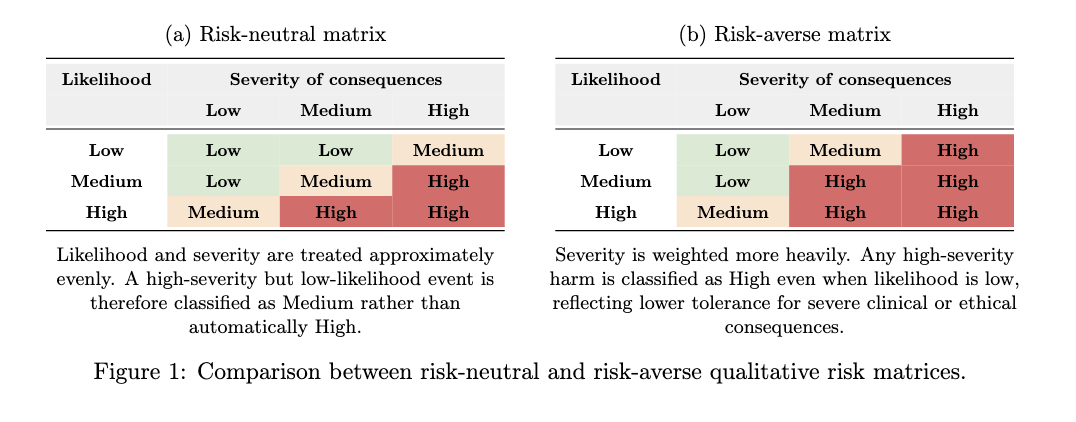
\includegraphics[width=\textwidth]{figures/risk_matrices.png}
    \caption{Qualitative likelihood-vs-severity matrices used in the risk assessment. The risk-neutral matrix (a) is used for commercial and operational risks; the risk-averse matrix (b) is used for clinical, safety and data-governance risks where severity is weighted more heavily.}
    \label{fig:risk-matrices}
\end{figure}

\subsection{Risk Assessment}

The principal risks identified in the report are recorded in \Cref{tab:risk-register} with their source or design limitation, the existing design or procedural control, and the residual limitation that must be verified during Phase 1.

\begin{table}[htbp]
    \centering
    \caption{Qualitative risk register for NeuroScreen.}
    \label{tab:risk-register}
    \footnotesize
    \begin{tabular}{p{2.6cm}p{3.6cm}cp{4cm}p{3.4cm}}
        \toprule
        \textbf{Risk} & \textbf{Source / design limitation} & \textbf{Initial} & \textbf{Mitigation / control} & \textbf{Residual limitation} \\
        \midrule
        \textbf{False negative / false reassurance} \emph{(Clinical)}
            & A ``low risk of mTBI'' output after a genuine mTBI could lead to injured athletes missing treatment.
            & High
            & NeuroScreen must use conservative thresholds, confidence scores and explicit warning statements.
            & NeuroScreen cannot rule out concussion or provide return-to-play clearance. \\
        \midrule
        \textbf{False positive / unnecessary referral} \emph{(Clinical)}
            & Conservative thresholds may incorrectly flag a non-concussed user as requiring further assessment.
            & Medium
            & Present abnormal outputs as ``further assessment recommended'' rather than as a diagnosis.
            & Some unnecessary referrals are acceptable in screening tools but may reduce trust or adoption if frequent. \\
        \midrule
        \textbf{Poor signal quality and image artefacts} \emph{(Technical)}
            & Poor fit, eyelash occlusion, glare, blur, low pupil--iris contrast, optical misalignment or ambient-light contamination may corrupt pupil and gaze measurements.
            & High
            & Use enclosed optics, fixed headset geometry, controlled NIR illumination, image-quality checks, signal-quality flag, confidence score and repeat-test logic.
            & Some users or conditions may produce no valid result; failure-to-test must be treated as safer than false reassurance. \\
        \midrule
        \textbf{Motion artefact and poor fit} \emph{(Operational)}
            & Pitch-side users may move during testing due to anxiety, instability, poor headset fit or recent injury, contaminating PLR, vergence or smooth-pursuit features.
            & High
            & IMU-based motion gating; reject or abort trials when motion exceeds threshold during critical windows; provide repeat-test prompts.
            & Motion rejection protects evidence quality but may reduce completion rate in real field use. \\
        \midrule
        \textbf{Physical user-safety failure} \emph{(Safety)}
            & Near-eye IR illumination, high display brightness, battery faults, overheating or electrical faults could expose the user to harm.
            & High
            & Controlled through the electronics safety architecture already specified: fixed illumination limits, calibrated brightness ceilings, watchdog/timeout behaviour, battery protection, fuel-gauge shutdown and conservative thermal design.
            & Controls are specified at design level but require verified bench and safety testing before Phase 1 human data collection. \\
        \midrule
        \textbf{Timing and synchronisation uncertainty} \emph{(Technical)}
            & PLR latency, pursuit phase lag and vergence timing depend on accurate stimulus and frame timing; the prototype does not yet use medical-grade hardware synchronisation.
            & Medium
            & High-frame-rate capture, timestamp logging, stimulus dwell periods, transition-frame exclusion, and validation against known timing events.
            & Timing uncertainty may bias extracted biomarkers until validated on the final integrated hardware. \\
        \midrule
        \textbf{ML, biomarker and population-validation gap} \emph{(Evidence)}
            & Model performance may not generalise across age, medication, fatigue, eye colour, iris pigmentation, prior TBI, visual history, or real pitch-side conditions.
            & High
            & Conduct governed Phase 1 dataset collection; lock model versions during validation; perform subgroup analysis; compare outputs against clinical assessment; maintain conservative claims.
            & Until clinical validation is complete, NeuroScreen can claim only decision support, not diagnostic accuracy. \\
        \midrule
        \textbf{Supply-chain and manufacturing variability} \emph{(Commercial)}
            & Measurement quality depends on camera selection, beamsplitter performance, optical alignment, display brightness, LED symmetry, calibration consistency and availability of strategic components.
            & Medium
            & Retain optical alignment, calibration, final integration and end-of-line testing in-house; use incoming inspection and second-source critical components where possible.
            & Scaling production may introduce device-to-device variability unless calibration and quality controls mature with volume. \\
        \bottomrule
    \end{tabular}
\end{table}


\section{Quality, Ethics and Sustainability}
\label{sec:ent-ethics}

\subsection{Quality Control System}

The EU conformity assessment in \Cref{sec:ent-regulatory-eu} requires a quality management system aligned with ISO~13485~\cite{iso13485}. It would, however, be unrealistic to propose full commercial quality management within the scope of the 3YP. A more appropriate strategy is a progressive quality-maturity guideline whose obligations rise with the phase of development.

\textbf{Phase 1.} This stage relies heavily on documentation of product iteration covering hardware revision, software version and operator notes. During the data-collection clinical trials, each test session must be traceable to a device identifier, protocol version, stimulus log, software build, preprocessing pipeline, model version and data-processing workflow, ensuring its defensibility with the HRA under the NHS approval pathway in \Cref{sec:ent-regulatory-uk}.

\textbf{Phase 2.} This stage assumes evidence integrity and moves to production-scale repeatability, which requires an ISO~13485-aligned QMS in which design requirements, risk controls, verification tests, supplier records, software releases and complaint feedback are formally linked~\cite{iso13485}. For this device, the highest-priority controls are optical alignment, camera focus, LED brightness, display luminance, IMU function, signal-quality thresholds, model versioning and result wording. Each unit released into Phase~2 pilots should pass an end-of-line test covering frame rate, binocular alignment, illumination symmetry, battery telemetry, thermal behaviour, Bluetooth result transmission, Wi-Fi upload and repeatability on a calibration target. Software and ML updates should move to a controlled release for each pilot period, with any change triggering regression testing and documented review. Pilot feedback, failed tests, discomfort, poor fit, confusing UI interactions and complaints should feed into a corrective-and-preventive-action (CAPA) process.

\subsection{Ethical Considerations}

\textbf{Inclusivity.} Oculomotor measurements vary with age, medication, fatigue, eye colour, iris contrast, prior TBI, visual impairment, and neurological or ophthalmological history~\cite{ortega2022medicalhistory,bergamini1998iriscolour}. The system must therefore be validated across the populations it claims to serve, as set out by Alderman et al.~\cite{alderman2024aitransparency}. For NeuroScreen, the intended user profile is restricted to 12--18 year-olds across a representative range of eye characteristics and medical and neurological history reflected in the dataset collected in Phase 1.

\textbf{Algorithmic transparency.} A non-expert operator does not need to inspect the model weights, but they do need to understand why a test was accepted, rejected or flagged based on signal-quality, motion and confidence indicators. This is sufficient transparency for the user to understand the limits of the result and when further medical assessment is required~\cite{alderman2024aitransparency,who_aiethics2021}.

\textbf{Pricing.} For a health-related product, pricing is not only a revenue model but also determines whether a device remains accessible at the point of need~\cite{who_pricing}. The commercial plan in \Cref{chapter:ent-business} deliberately does not gate emergency screening behind a recurring consumer subscription, instead relying on a one-off hardware sale with an optional institutional subscription for additional administrative features. This is ethically stronger than charging parents continuously for the right to use a device that may only be needed unpredictably after injury.

\subsection{Lifecycle, Environmental Impact and Sustainability}

A full lifecycle assessment (LCA) sits alongside the EU MDR technical file, risk management, post-market surveillance and CE-marking pathway. The appropriate framework for that future assessment is ISO~14040/14044, which defines LCA in terms of goal and scope, life-cycle inventory, impact assessment and interpretation~\cite{iso14040}.

The relevant product lifecycle has five stages: component sourcing, assembly and calibration, use, maintenance and end-of-life. Components such as electrical and electronic assemblies, camera modules, the display, PCB assemblies, optical components, the LiPo battery, enclosure materials and straps must therefore be selected with the EU RoHS restrictions on hazardous substances, REACH chemical obligations, and EU battery requirements in mind~\cite{eu_rohs,eu_reach,eu_batteries}.

Assembly and initial calibration are enforced by end-of-line testing with periodic functional checks for battery ageing, cleaning, storage effects and software updates, as set out in the quality plan above. Maintenance is supported by replaceable straps, facial interface, battery, camera modules, illumination board and (potentially) the display, with any replacement triggering device recalibration.

End-of-life can be distinguished between reusable, refurbishable and waste components. Returned Phase~1 or Phase~2 devices may still be useful for training or software testing even if unsuitable for commercial redeployment. Batteries require controlled disposal under the EU battery regulation~\cite{eu_batteries}; PCBs, cameras and display electronics enter WEEE-compliant waste streams~\cite{eu_weee}; and packaging must comply with the EU packaging-waste regulation~\cite{eu_packaging}.

The main environmental impacts are concentrated in electronics manufacture, battery replacement and disposal, and cloud data transfer. The sustainability strategy is therefore to adopt design decisions that reduce future impact: modular repair, replaceable batteries, reusable or refurbishable returned units, and compliant disposal of electronic waste. This becomes especially important in Phase~3, where wider amateur-sport distribution increases the number of devices outside direct company control.
